\documentclass[12pt,fleqn]{article}\usepackage{../common}
\begin{document}
Lineer Cebir - Ders 1

Ilk dersimize hosgeldiniz, ben Gilbert Strang. Lineer cebirin cozmeye
calistigi en temel problem bir lineer denklem sistemini cozmektir. Bu
baglamda mesela en genel durum ``bilinmeyen ve denklem sayisinin birbirine
esit oldugu'' durumdur, ki bu ``guzel durum'' olarak nitelenebilir. Boyut
$n \times n$ olunca bu durumda oluyoruz. Ama diger durumlari da
isleyecegiz. 

Dersin kavramlarini anlamak icin  ``satir bakisi''na basvuracagiz, bu
durumda her denkleme teker teker bakiyoruz gibi olacak, dersimizde pek cok
kez kullanacagimiz $A$ matrisimiz olacak mesela, ve bu matrisin satirlarin
her denklemin degiskenlerinin katsayilarina tekabul edecek.

Kolon bakis acisi belki daha once gormediginiz bir aci olacak, bu durumda
her kolon ayri ayri islenecek. 

Cebirsel bakis acisi ise tum matrisi, bu durumda $A$, ayni anda ele alacak.

Guzel durumdan baslayalim; iki bilinmeyen, iki denklem.

$$ 2x - y = 0 $$

$$ -x + 2y = 3 $$

Katsayilari matrise tasiyalim

$$ 
\left[\begin{array}{cc}
2 & -1 \\
-1 & 2
\end{array}\right]
\left[\begin{array}{c}
x \\
y
\end{array}\right]
=
\left[\begin{array}{c}
0 \\
3
\end{array}\right]
 $$

Soldaki matrise ben cogunlukla $A$ derim, sonra icinde bilinmeyenleri
tasiyan $x$ vektoru koyarim, ki bazilari bunu vektor oldugu icin koyu
renkte $\mathbf{x}$ olarak ta yazar, ve sonra bir vektor daha, ki buna ben
cogunlukla $b$ derim, yani sonuc soyle olur,

$$ A x = b $$

Simdi satir bakisina basvuralim. Grafik olarak dusunelim, hangi noktalar
$2x - y = 0$ denklemini tatmin eder? Orijin $(0,0)$ noktasi bunlardan biri,
bir digeri $x=1,y=2$. Bunlari cizgi ile birlestirip cizgiyi sonsuza uzatirsak,

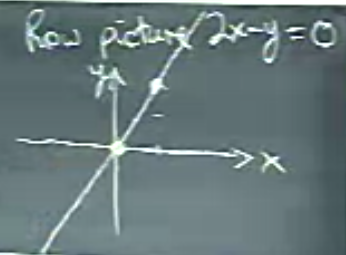
\includegraphics[height=4cm]{1_01.png}

Ikinci denklemi dusunelim, bu denklem orijinden gecmeyecek. $y$ sifir
olsaydi $x$ nereden gecerdi..? $x=-3$ noktasindan. $x=-1$ ise, $y$ nedir?
$y=1$. Artik ikinci cizgiyi cizebiliriz,

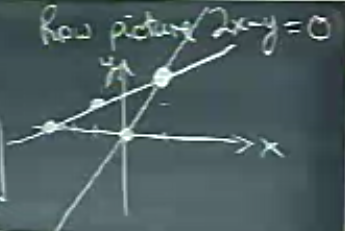
\includegraphics[height=4cm]{1_02.png}

Her iki cizgi $x=1,y=2$ noktasinda bulustu (hoca o noktayi daha onceden
tahtaya koymustu ama buna bir ``hazir raslanti'' diyelim). Bu bulusma
noktasi her iki denklemi tatmin eden sistemin cozum noktasidir.

Kolon bakisina gelelim. Bu bakisa gore

$$ 
x
\left[\begin{array}{r}
2 \\
-1
\end{array}\right]
+
y
\left[\begin{array}{r}
-1 \\
2
\end{array}\right]
=
\left[\begin{array}{r}
0 \\
3
\end{array}\right]
$$

Bu bakis acisi bize ne soyluyor? Bir anlamda diyor ki ``esitligin solundaki
iki vektoru oyle bir sekilde kombine et ki bu lineer kombinasyon sonucu
esitligin sag tarafini versin''. Bu operasyon, islem lineer cebir dersinin
en temel islemidir - kolonlarin lineer kombinasyonu. 

Kolonlari vektorel olarak cizelim, bilindigi gibi bir vektor orijinden
cikan bir yonu ve buyuklugu olan bir seydir. Birinci kolon 2 saga 1 asagi
gitmeli, ikincisi bir sola 2 yukari gitmeli. Cizince,

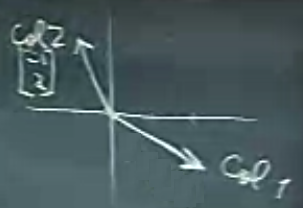
\includegraphics[height=4cm]{1_03.png}

Peki bu vektorleri nasil ``birlestirelim'' yani hangi katsayilarla carpip
toplayalim ki $[3,0]^T$ sonucunu elde edelim? Not: Burada devrik isaretini
kullandik cunku satir vektorunun devrigini alinca kolon vektoru olur,
yazarken o sekilde yazdik cunku baska turlu yazi icine rahat koymak mumkun
olmayacakti. 

Neyse, kombine etmek toplamaktir, o zaman ikinci kolonu alip birinciye
ekleyelim, vektor aritmegitinde toplamak bir vektoru digerinin bittigi
noktadan baslatmak demektir, bir tane (yani katsayi 1 ile) ikinci vektoru
birinciye ekleyince

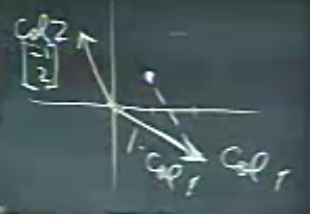
\includegraphics[height=4cm]{1_04.png}

Cozum noktasina erisemedik daha, 2 tane ekleyince,

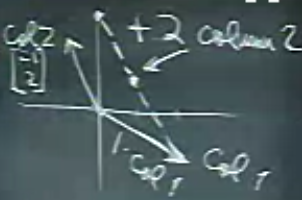
\includegraphics[height=4cm]{1_05.png}

Cozume eristik. Cozum $y$ ekseni uzerinde 3,0 noktasi. Bu noktaya bir
lineer kombinasyon yaparak eristik. ``Dogru'' lineer kombinasyon bize
sonucu verdi. 

Kendimize sunu soralim: {\em butun} lineer kombinasyonlar bize neyi
verirdi? Bu cok onemli bir soru, uzerinde iyi dusunelim, cunku bu konu
tekrar tekrar karsimiza cikacak. Tum kombinasyonlar derken tum $x,y$'lerin
doguracagi kombinasyonlar; bu sekilde esitligin sag tarafi ne olursa olsun
onu temsil edebilirdik. Yani bu tum kombinasyonlar tum bir duzlemi (plane)
doldururdu. Bunu bir kenara koyalim, konuyu ileride daha detayli olarak
inceleyecegiz.

3 Boyut

$$  2x - y = 0  $$

$$ -2x + y - z = -1 $$

$$ -3y + 4z = 4 $$

Bu sistemi nasil anlariz? Ne gorduk: satir bakisi, kolon bakisi. Matris
formuna bakalim, 

$$ A = 
\left[\begin{array}{rrr}
2 & -1 & 0 \\
-1 & 2 & -1 \\
0 & -3 & 4 
\end{array}\right]
,
b = 
\left[\begin{array}{r}
0  \\
-1 \\
4  
\end{array}\right]
 $$

Satir bakisi, ustteki ikinci denklemi alalim, grafigi neye benzer?
Orijinden gecen bir sey yok, cunku $0,0,0$ bir cozum olamaz. Cozum neye
benzer? Elimizde bir lineer denklem var ise uc boyutta bu denklemi cozen
tum noktalar bir duzlem (plane) olustururlar. Hoca diyor ki ben Rembrandt
degilim, kabaca bir duzlem cizecegim, 

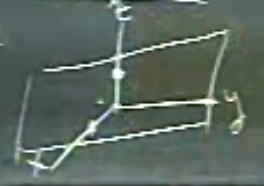
\includegraphics[height=4cm]{1_06.png}

Birinci denklem neye benzer? $z$ belirtilmemis, demek ki herhangi bir sey
olabilir, geri kalanlar yine bir duzlem olustururlar. Mesela alttaki gibi

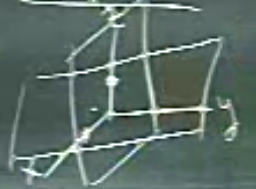
\includegraphics[height=4cm]{1_07.png}












\end{document}
